\documentclass[11pt,a4paper,oldfontcommands]{memoir}
\usepackage[utf8]{inputenc}
\usepackage[T1]{fontenc}
\usepackage{microtype}
\usepackage[dvips]{graphicx}
\usepackage{xcolor}
\usepackage{todonotes}
\usepackage{times}
\usepackage{amsmath}
\usepackage{natbib}
\usepackage{array}



\usepackage{listings}

\lstset{
  language = C,
  basicstyle=\small,    % the size of the fonts that are used for the code
  stepnumber=1,                           % the step between two line-numbers. If it is 1 each line will be numbered
  numbersep=10pt,                         % how far the line-numbers are from the code
  tabsize=2,                              % tab size in blank spaces
  extendedchars=true,                     %
  breaklines=true,                        % sets automatic line breaking
  captionpos=b,                           % sets the caption-position to top
  mathescape=true,
  stringstyle=\color{white}\ttfamily,
  showspaces=false,           
  showtabs=false,             
  xleftmargin=17pt,
  framexleftmargin=17pt,
  framexrightmargin=17pt,
  framexbottommargin=5pt,
  framextopmargin=5pt,
  showstringspaces=false     
 }

\newcommand\typestyle{\rmfamily\mdseries\upshape}
\newcommand\addtypes[1]{%
  \lstset{morekeywords=[3]{#1}}}

\usepackage[
breaklinks=true,colorlinks=true,
%linkcolor=blue,urlcolor=blue,citecolor=blue,% PDF VIEW
linkcolor=black,urlcolor=black,citecolor=black,% PRINT
bookmarks=true,bookmarksopenlevel=2]{hyperref}

\usepackage{geometry}
% PDF VIEW
% \geometry{total={210mm,297mm},
% left=25mm,right=25mm,%
% bindingoffset=0mm, top=25mm,bottom=25mm}
% PRINT
\geometry{total={210mm,297mm},
left=20mm,right=20mm,
bindingoffset=10mm, top=25mm,bottom=25mm}

\usepackage{bytefield}
\usepackage{msc}

\OnehalfSpacing
%\linespread{1.3}

%%% CHAPTER'S STYLE
\chapterstyle{bianchi}
%\chapterstyle{ger}
%\chapterstyle{madsen}
%\chapterstyle{ell}
%%% STYLE OF SECTIONS, SUBSECTIONS, AND SUBSUBSECTIONS
\setsecheadstyle{\Large\bfseries\sffamily\raggedright}
\setsubsecheadstyle{\large\bfseries\sffamily\raggedright}
\setsubsubsecheadstyle{\bfseries\sffamily\raggedright}


%%% STYLE OF PAGES NUMBERING
%\pagestyle{companion}\nouppercaseheads 
%\pagestyle{headings}
%\pagestyle{Ruled}
\pagestyle{plain}
\makepagestyle{plain}
\makeevenfoot{plain}{\thepage}{}{}
\makeoddfoot{plain}{}{}{\thepage}
\makeevenhead{plain}{}{}{}
\makeoddhead{plain}{}{}{}


\maxsecnumdepth{subsection} % chapters, sections, and subsections are numbered
\maxtocdepth{subsection} % chapters, sections, and subsections are in the Table of Contents


%%%---%%%---%%%---%%%---%%%---%%%---%%%---%%%---%%%---%%%---%%%---%%%---%%%

\begin{document}

%%%---%%%---%%%---%%%---%%%---%%%---%%%---%%%---%%%---%%%---%%%---%%%---%%%
%   TITLEPAGE
%
%   due to variety of titlepage schemes it is probably better to make titlepage manually
%
%%%---%%%---%%%---%%%---%%%---%%%---%%%---%%%---%%%---%%%---%%%---%%%---%%%
\thispagestyle{empty}

{%%%
\sffamily
\centering
\Large

~\vspace{\fill}

EPL-2014 384\\
{\huge 
To be defined
}

\vspace{2.5cm}

{\LARGE
Quentin Devos \\
Loïc Fortemps de Loneux
}

\vspace{3.5cm}

A thesis submitted in partial fulfillment for the\\
Master in Computer Science Engineering\\[1em]
in the\\[1em]
Louvain School of Engineering\\
Université Catholique de Louvain

\vspace{3.5cm}

Supervisors: \\
            Prof. Olivier Bonaventure\\
             Prof. Olivier Pereira

\vspace{\fill}

June 2015

%%%
}%%%

\cleardoublepage
%%%---%%%---%%%---%%%---%%%---%%%---%%%---%%%---%%%---%%%---%%%---%%%---%%%
%%%---%%%---%%%---%%%---%%%---%%%---%%%---%%%---%%%---%%%---%%%---%%%---%%%

\tableofcontents*
\clearpage

\listoffigures*
\clearpage

%%%---%%%---%%%---%%%---%%%---%%%---%%%---%%%---%%%---%%%---%%%---%%%---%%%
%%%---%%%---%%%---%%%---%%%---%%%---%%%---%%%---%%%---%%%---%%%---%%%---%%%

%\chapter{Protocol Design}\label{chap:design}

In this chapter, we will explore the different additions and modifications made to DTLS to support the Multipath capability. These changes are categorized in three groups:
\begin{itemize}
\item Advertising the extension and the interfaces
\item Establishing secure sub-flows without introducing attacks vectors
\item Gathering and exchanging statistics data about the health of each flow, regardless of the others. 
\end{itemize}


\section{Multipath advertisement}

Our main purpose is to set up this protocol as an extension of DTLS. In this way, we can reuse as much as possible the principles established by Rescorla and Modadugu in \cite{modadugu2004design}. This also explains why we tried not to change the existing DTLS frames and to add instead new frames for new usages.

\subsection{Extension discovery}\label{sec:helloext}

The first step, and the first requirement, was to remain compatible with the standard DTLS client and server. To do that, the MPDTLS extension discovery is made through a new entry in the extensions list of the \texttt{ClientHello} and \texttt{ServerHello} messages. If a MPDTLS-unable server receives a \texttt{ClientHello}, it will ignore the option as it is specified in the TLS 1.3 specifications (\texttt{draft-ietf- tls-tls13}\cite{draft-tls13}). This option is carried as any other TLS Hello Extension (Section 7.3.2.5 from the same draft) with the following format:

\addtypes{ExtensionType, byte, Extension}
\begin{lstlisting}[caption=MultiPath DTLS Extension structure, label=lst:extension]
struct {
  ExtensionType extension_type;
  byte          extension_length[2];
  byte          extension_data[1];
} Extension;

enum {
    mpdtls_extension(TBD, 42 in dev), (65535)
} ExtensionType;
\end{lstlisting}

This extension is simply carrying a byte indicating if the host supports MPDTLS or not (so it carries \texttt{0x01} or \texttt{0x00} respectively).

After the exchange of the \texttt{HelloVerifyRequest} and \texttt{ClientHello} with Cookie, the server will send back a \texttt{ServerHello} containing the same extension if it wants to support MPDTLS features. Besides this MPDTLS extension discovery, the handshake is exactly the one from DTLS, keeping the handshake as light as possible.

\subsection{Advertising interfaces}
\label{sec:advertise}

Like in MPRTP (see Section \ref{sec:mprtp-advertise}), we can explore 2 options for the addresses advertisement : in-band or out-of-band signalling. "In-band" means we use the same protocol (in this case DTLS) to exchange our addresses while "out-of-band" will imply another protocol that could be reliable for instance. For MPDTLS, we made the choice to consider only the in-band communication for the following reasons : 

\begin{itemize}
\item Lower overhead: we don't need any additional protocol or to set up another channel of communication.
\item The addresses must be communicated securely. We already have a secure channel with DTLS, it is thus unnecessary to do another handshake with TCP/TLS.
\item The reliability is not a strong requirement. The message carrying all the addresses may be lost, this is not vital for the communication. Moreover, with a small retransmission strategy, it will eventually reach the destination.
\end{itemize}


Once the handshake is finished and the initial flow is established, the two hosts can advertise new interfaces available for other sub-flows. This is done within the \texttt{ChangeInterfaceMessage} (CIM), a packet carrying multiple addresses. This packet is carried as a DTLS fragment and thus is protected in the same way the Application Data are. The structure of the \texttt{CIM} packet is shown in the Listing \ref{lst:cimformat}. We use 16 bytes for the address to be IPv6 compliant. IPv4 addresses can be mapped to/from IPv6 format following \texttt{RFC4291}\cite{rfc4291}. This mapping allows us to keep the size of the packet relatively small when you compare it with the one from MPRTP (Listing \ref{lst:mprtcp-advertisement}). Of course we don't support DNS name. It could be interesting to let the other host do the DNS resolution but for now we think it is not needed. We can always extend the design if a need for other kind of interface advertisement is observed.

\addtypes{ContentType,ProtocolVersion,uint16,uint48,uint64,byte,ChangeInterfaceMessageFragment,DTLSPlainText, NewAddress,select,case}
\begin{lstlisting}[caption=Change Interface Message, label=lst:cimformat]
struct {
    ContentType type;
    ProtocolVersion version;
    uint16 epoch;
    uint48 sequence_number;
    uint16 length;
    select (ContentType) {
        case change_interface: ChangeInterfaceMessageFragment; // New field
    } fragment;
} DTLSPlaintext;

enum {
    change_interface(TBD, 42 in dev), (255)
} ContentType;

struct {
    byte reply;
    if (reply) {
        uint48 ack;
    }
    byte number_addresses[2];
    NewAddress addresses<1..2^16-1>;
} ChangeInterfaceMessageFragment;

struct {
    byte address[16];
    uint16 port;
} NewAddress;
\end{lstlisting}

The \texttt{CIM} contains all the addresses a host wants to share. We decided to always transmit all the addresses to provide redundancy. Also, to be sure we do not lose potential bandwidth, the \texttt{CIM}s are retransmitted in case of loss and so are acknowledged. To avoid wasting resources, we use the acknowledgement to transmit the list of addresses of the receiving host. This way, we are sure that each host knows the exact configuration of the other at any time (once the first host received the acknowledgement). This strategy has also been chosen for the retransmission in MPRTP \cite{singh-avtcore-mprtp}.

An example of the \texttt{CIM} exchange is shown in the Figure \ref{fig:CIMexchange}. The message is structured as follows: the fact that it is an acknowledgement or not (reply bit), the total number of interfaces we are advertising and the list of interfaces (following format presented in Listing \ref{lst:cimformat}). For the sake of clarity, the DTLS informations (such as the epoch, version,\dots) are not represented on Figure \ref{fig:CIMexchange} and the sequence numbers are shown between chevrons.

\begin{figure}[!ht]
\centering
\begin{msc}[r]{MultiPath-DTLS Addresses announcement}

\setlength{\instfootheight}{0em}
\setlength{\instheadheight}{0em}
\setlength{\instdist}{0.7\linewidth}
\setlength{\levelheight}{3em}

\declinst{client}{Client}{}
\declinst{server}{Server}{}

\lost[r]{ChangeInterfaceMessage[[reply=1], 2, client1, client2 ] - <1>}[t]{}{client}[8]
\settimeout{}{client}[1]
\nextlevel
\mess{ChangeInterfaceMessage[[reply=1], 2, client1, client2] - <2>}[t]{client}[0]{server}[1]
\nextlevel
\mess{ChangeInterfaceMessage[[reply=0,ack=2], 1, server1] - <1>}[b]{server}[1]{client}[1]
\nextlevel
\nextlevel

\end{msc}
\caption{Example of Change Interface Message use}
\label{fig:CIMexchange}
\end{figure}

To avoid an infinite exchange of \texttt{CIM}s, a reply bit is needed and placed into the header of \texttt{CIM} to differentiate a new message from an acknowledgement to a previous one. Also, to know which CIM request is acknowledged, its DTLS sequence number is added in the response. The client must store the sequence number of the last CIM emitted. When an \texttt{CIM} is received but the host realizes the stored sequence number doesn't match the received ack, it must retransmit the \texttt{CIM}.

\subsection{Retransmission strategy}

A CIM message must be retransmitted if the reply is not received because the packet may be lost. How do we monitor the reception ? We could use a timeout to retransmit after a certain period of time. But if the other host is definitely dead, we will send packets for nothing before we figure out.

We could point out the fact that the knowledge of the interfaces is only needed when the host is really using them (i.e. sending packets). Therefore, we could think of a mechanism which retransmits only when there is evidence that the other is still alive : when we receive application data packets. When the first CIM is sent, we set a flag to 1. This flag is put back to 0 as soon as we receive a CIM with \verb$reply = 0$. But if we receive an application data with the flag still on, we process the data and retransmit the last CIM. An example is presented on Figure \ref{fig:CIMexchange2}.

\begin{figure}[!ht]
\centering
\begin{msc}[r]{MultiPath-DTLS Addresses announcement RTX}

\setlength{\instfootheight}{0em}
\setlength{\instheadheight}{0em}
\setlength{\instdist}{0.7\linewidth}
\setlength{\levelheight}{3em}

\declinst{client}{Client}{}
\declinst{server}{Server}{}

\lost[r]{ChangeInterfaceMessage[reply=1, 2, client1, client2]}[t]{}{client}[7]
\nextlevel
\mess{ApplicationData}[t]{server}[0.3]{client}[1]
\nextlevel
\mess{ChangeInterfaceMessage[reply=1, 2, client1, client2]}[t]{client}[0.25]{server}[1]
\nextlevel
\mess{ChangeInterfaceMessage[[reply=0], 1, server1]}[b]{server}[1]{client}[1]
\nextlevel
\nextlevel

\end{msc}
\caption{Example of Change Interface Message Retransmission}
\label{fig:CIMexchange2}
\end{figure}

Of course if some packets were already on the line before the server has received the CIM, we will retransmit many times the CIM and therefore waste bandwidth.

Our solution is somehow a mix between the pure timeout and the direct retransmission after every packet. When we first send the \texttt{CIM}, we store a timestamp in a variable. For every packets received, we check if the elapsed time is enough and we retransmit the packet and reset the timestamp to the current time. The "enough" is customizable, we could set a default value of 2 RTT for \texttt{CIM} retransmission. The main benefit of checking only when we receive packets is that we don't waste bandwidth for dead links and we don't need parallelization mechanism (e.g. interruptions).

This strategy will be used for all retransmission of control packets with possibly different thresholds for the timers.

\section{Secure sub-flows setup}\label{sec:setupflow}

In the first design of our protocol, we didn't use any handshake to attach new sub-flows to the global connection. Instead, we were creating all the possible sub-flows by combining the host and remote addresses, directly initializing the sockets in connected mode. However, this solution is not suitable in various situations, like NAT-traversals or short-living interfaces. 

Other multipath protocols don't need to explicitly start a new flow. That's the case for MPRTP, the interfaces are just advertised and all possible combinations of 2 interfaces are then acceptable. But MPRTP doesn't have any security concerns as we do.

Using not connected sockets could present a potential weak point for a DoS (Denial of Service) attack. If an attacker could guess IP addresses of the server, she can send garbage under the form of traditional DTLS packets. This could get computation costly since it forces the server to establish the packet authenticity and involves cryptographic operations. This is cheaper if we use connected sockets because packets coming from other addresses or ports than the connected ones are immediately dropped by the UDP stack. Also, this problem does not appear when the involved packets are not cryptographically signed, like the handshake packets. The solution presented in the Section \ref{sec:breakbeforemake} allows to overlook this issue as it is based on the shortened DTLS handshake.

To address this issue, we define three scenarios of sub-flow creation and the solutions to cope with.

\subsection{Make-before-break sub-flows}
\label{sec:mbf}

We want to set up a new sub-flow when we have at least one other sub-flow alive. In this situation, we will use the secure communication already established to negotiate the opening of a new connection. Only when the negotiation is completed, a new socket will be created and connected on both side, avoiding any possible DoS attack on the new interface.

To carry this request, we need a new type of packet : \texttt{wantConnect}, whose structure is shown on Listing \ref{lst:WantConnect}.

\addtypes{WantConnectFragment}
\begin{lstlisting}[caption= WantConnect message, label=lst:WantConnect]
enum {
    want_connect(TBD), (255)
} ContentType;

struct {
    NewAddress addr_src;
    NewAddress addr_dst;
    byte opts;
} WantConnectFragment;

struct {
    byte address[16];
    uint16 port;
} NewAddress;
\end{lstlisting}

The field \texttt{opts} can be used to specify options for the incoming connection. The first bit of opts is telling if the host accepts or refuses the connection and will only be used in the reply. A second bit is used as the backup flag. When this flag is set to 1, it means we want to use this interface only if it is the only possible choice to keep the connection running. Typically, this would be the case for a 4G/LTE interface on a phone because it costs much more than the Wi-Fi. The 6 remaining bits are unused for now but may be useful in the future.

The host who received a \texttt{wantConnect} must acknowledge the reception thanks to a \texttt{wantConnect Ack} packet (see Listing \ref{lst:WantConnectAck}). Messages can be lost and we need to know to which Packet the acknowledgement is referring to, so we include the sequence number of the corresponding packet (i.e. DTLS sequence number). The options are also included to give the opportunity to the other host to accept or deny some of them. In particular, the first bit is set to 1 if the host refuses the connection and zero otherwise.

\addtypes{WantConnectAckFragment}
\begin{lstlisting}[caption= wantConnectAck message, label=lst:WantConnectAck]
enum {
    want_connect_ack(TBD), (255)
} ContentType;

struct {
    uint48 ack_seq;
    byte opts;
} WantConnectAckFragment;
\end{lstlisting}

Figure \ref{fig:Handshake1} presents how it will take place when a server has 2 interfaces and the client only one. First the traditional DTLS handshake is established between the client and the public interface of the server (S1). By a \texttt{CIM} exchange, the client is aware of the existence of a second interface (S2). He then sends a \texttt{wantConnect} request and if this message is correctly received, the server will set up his second interface to receive packets from the client. After this exchange, heartbeat messages will take place to assess the availability of the link. The frequency must be defined according to experimentation, at this point we recommend to send a heartbeat message at least every 5s. The implementation must use a back-off strategy to prevent waisting resources on a dead link. If for some reasons, the interface is not reachable from the client, then the server will find out it never receives any heartbeat response and will close the socket. Otherwise, a new sub-flow has been set up and both hosts can use it to communicate securely. 


\begin{figure}[!ht]
\centering
\begin{msc}[r]{MultiPath-DTLS handshake make-before-break}

\setlength{\instfootheight}{0em}
\setlength{\instheadheight}{0em}
\setlength{\instdist}{0.33\linewidth}
\setlength{\levelheight}{3em}

\declinst{client}{Client (C)}{}
\declinst{server1}{Server1 (S1)}{}
\declinst{server2}{Server2 (S2)}{}

\mess{DTLS Hanshake}[t]{client}[0.5]{server1}[0]
\nextlevel
\mess{DTLS Hanshake}[t]{server1}[0.5]{client}[0]
\nextlevel
\mess{CIM[2, S1, S2, reply=1]}[t]{server1}[0.1]{client}[1]
\nextlevel
\mess{CIM[1, C, reply=0]}[b]{client}[0.8]{server1}[1]
\nextlevel[2]
\mess{WantConnect[C,S2,op]}[t]{client}[0.1]{server1}[1]
\nextlevel
\mscmark{connected socket}{server2}
\mess*{}{server1}{server2}[0]
\mess{WantConnectAck[op]}[t]{server1}[0.3]{client}[1]
\nextlevel
\mscmark[br]{connected socket}{client}
\nextlevel
\mess{HeartbeatRequest}[t]{client}[0.6]{server2}[1]
\nextlevel
\mess{HeartbeatResponse}[b]{server2}[0.4]{client}[1]
\nextlevel[2]

\end{msc}
\caption{Example of new sub-flow establishment when another connection is alive}
\label{fig:Handshake1}
\end{figure}

When another connection is available, this is the best method to establish a new sub-flow since it is way faster than a complete handshake. Note that the two new messages introduced are secured as any other DTLS message and therefore cannot be forged or replayed.


\subsection{Break-before-make sub-flows\label{sec:breakbeforemake}}
Unfortunately, the solution presented in the previous section is not applicable in every situation; for instance, when a smartphone is connected with its Wi-Fi interface and the access point becomes out of range for any reason. The smartphone will then toggle the 4G interface. It cannot use the procedure explained in the previous section as it does not have an active sub-flow anymore. To solve this problem, the smartphone can simply use the Session Resumption mechanism available in (D)TLS, resuming on both sides the state of the session as before the link failure. It is also important that the smartphone warns the server that the Wi-Fi interface is no more available by sending a \texttt{CIM} as soon as it re-establishes the connection. This use case is presented on Figure \ref{fig:dtls-sessionresumption}.

\begin{figure}[!ht]
\centering
\begin{msc}[r]{MultiPath-DTLS session resumption}

\setlength{\instfootheight}{0em}
\setlength{\instheadheight}{0em}
\setlength{\instdist}{0.33\linewidth}
\setlength{\levelheight}{3em}

\declinst{client1}{Client2 (4G)}{}
\declinst{client2}{Client1 (WiFi)}{}
\declinst{server}{Server}{}

\mess{DTLS Hanshake}[t]{client2}[0.5]{server}[0]
\nextlevel
\mess{DTLS Hanshake}[t]{server}[0.5]{client2}[0]
\nextlevel
\mess*{Share session ID}{client2}{client1}[0]
\nextlevel
\condition{WiFi Off}{client2}
\nextlevel
\stop{client2}
\condition{4G On}{client1}
\nextlevel
\mess{ClientHello (with session id)}[t]{client1}[0.5]{server}[0]
\nextlevel
\mess{HelloVerifyRequest}[t]{server}[0.5]{client1}[0]
\nextlevel
\mess{ClientHello (with session id, cookie)}[t]{client1}[0.5]{server}[0]
\nextlevel
\mess{ServerHello (with same session id)}[t]{server}[0.5]{client1}[0]
\nextlevel
\mess{ChangeCipherSpec}[t]{server}[0.5]{client1}[0]
\nextlevel
\mess{ChangeCipherSpec}[t]{client1}[0.5]{server}[0]
\nextlevel
\mess{ChangeInterface(Client2)}[t]{client1}[0.5]{server}[0]
\nextlevel
\mess{ChangeInterface(Server)}[t]{server}[0.5]{client1}[0]
\nextlevel[2]

\end{msc}
\caption{Example of how session resumption takes place}
\label{fig:dtls-sessionresumption}
\end{figure}

Note this is only possible because Client1 and Client2 are the same machine and therefore share the session ID given by the server. The handshake is faster if the session is still on the server's cache because no certificate exchange is needed and the master key is the same as before.

This solution presents the same security properties than the standard Session Resumption proposed in the \texttt{RFC5246}\cite{rfc5246}, Section 7.4.1.2. The RFC doesn't explicitly limit the session resumption to come from the same IP/port as before but it appears that some implementation do it. It was the case for Firefox and was criticized as a bug by N. Modadugu who is the co-author of DTLS\footnote{\url{https://bugzilla.mozilla.org/show_bug.cgi?id=415196}}. It can't be considered as a weakness since even if an attacker can steal the session ID, he doesn't know the master key and therefore won't be able to generate a correct \texttt{ChangeCipherSpec}.

If the server clears the session cache in the meantime, the full DTLS handshake will take place and the server and the session will start without any other known remote interface. This is another reason to impose a \texttt{CIM} emission as soon as the sub-flow is up.

Moreover, to make this solution working, a thread or a process must be constantly listening the interface even if a connection is already initiated. This was not a requirement for the \textit{WantConnect} solution.

Finally, we can say that this last solution is more generic than the previous one, as it can be used in every situation, when the \texttt{WantConnect} can only be used if a sub-flow is already established. Nevertheless, this method could potentially complicate the implementation if a flow is up and you try to do session resuming with another flow. You will have two separated DTLS sessions and the expected behavior is to merge these two into only one session. It would imply to use some communication channel between processes (shared memory for instance) and to merge objects together. But our experience working with an SSL/TLS library shows it won't be easy. So the best solution to establish new flows when at least one other flow is alive stays the \texttt{WantConnect} method.

\subsection{NAT-traversal sub-flows}

However, an overview of the possible scenarios would not be complete without taking into account the NAT that are widely deployed in home networks. To do so, we can reevaluate the solutions proposed in the previous sections to see if they can fit in presence of NAT. For the sake of simplicity and brevity, we only will consider the situations where only one host is behind a NAT.



\subsubsection{Make-before-break}

Unfortunately, the initialization of new subflows as described in \ref{sec:mbf} is not possible as it is if one host is behind a NAT. Indeed to create a connected socket, one host must know both the IP address and the port number of the other host. While the IP address may be obtained by some external online tool, the port is attributed by the NAT when the flow is created. So, the NATed host has no clue to guess that port number.

To perform efficiently NAT traversal, we must rely on an external protocol for session establishment. Such a tool is available under the name of Session Traversal Utilities for NAT(STUN) and is described in RFC 5389\cite{RFC5389}. It uses an external server with a public IP to play the role of intermediary and get public IP and port number for a particular session.

Other protocol actually delegate this task even if no NAT is present. This is the case for RTP and thus MPRTP, the IP addresses and ports are obtained typically via Session Initiation Protocol (SIP) \cite{RFC3261}.

Therefore, we let the application obtain the public IP address and the port of every interface via another protocol. In the prototype we have developed to test our implementation this feature has not been implemented since the objective was not to produce a commercial tool to use at home.


\subsubsection{Break-before-make}
The session resumption method is not altered by the NAT. The only constraint is that the handshake must be initated by the NATed host, to allow the NAT-holing and the correct address discovery.


\section{Feedback on sub-flow}
\label{sec:mpdtls-feedback}

Last but not least, each packet must be sent on a single flow. Thus, one needs to dispatch the packets over the sub-flows, and this is the role of the scheduler. But, to be able to do its work efficiently, the scheduler must be aware of the sub-flows health. To implement this new feature, we propose to add to DTLS a feedback mechanism, gathering various information such as the Forward delay, the drop rate of the link or the global reorder rate. Crossing the information we receive from different sub-flows will allow the scheduler to dispatch packets efficiently.

\subsection{Forward delay estimation}
\label{sec:forward-delay}
The transmission delay is an important measure when we want to balance a load over multiple flows. But, in our first design attempt, we used the RTT to measure this delay, estimating the one-way delay to the half of the RTT. However, as a majority of the links over the Internet are asymmetric, it sometimes leads to major differences between the real one-way delay and our estimation. We thus needed to reconsider the way to compute the delay.

The most intuitive way to compute the time taken to realize a task is to compare the time before its beginning and after its completion, which makes no sense when it comes over the network. As the task starts on one host and finishes on the other, we are subject to the clock synchronisation.

However, Fei Song et Al. propose in \cite{song2009estimator} a practical solution that suits our needs. The idea is simple: we don't need to know the exact One-way delay of a subflow, we just need to be able to compare the delays between the different sub-flows. So, we can compute the transmission delay of a flow as the difference between the sending time and the receiving time, with a $\Delta T$ term being the clock desynchronization between the two hosts. This $\Delta T$ is only the clock difference that could exist between the two actors of the connection and it does not hide any delay or jitter caused by the transmission itself. As the two end-points of all the sub-flows are the same, this $\Delta T$ is assumed to be constant over all the sub-flows.

Once we know how to estimate the forward delay of each subflow, or at least how to rank them on this criteria, we can easily create a mechanism to compute this estimation, it is illustrated in the Figure \ref{fig:forwardDelayComputation}. To avoid overhead on each DTLS AppData packets, we took the decision to use new dedicated packets to compute the forward delay. Each host will periodically send probe packet containing the current timestamp. When the other host receives it, it can compute the transmission delay modulo $\Delta T$. For the sake of simplicity, only the average of the delay computed will be transmitted in the \texttt{feedback} report, as presented in Section \ref{sec:feedbackReport}. The $\Delta T$ is considered constant over time because the clocks are increasing in the same way on all the hosts. As $\Delta T$ is constant, it does not introduce deviation in the calculation of the transmission delay average. 

\begin{figure}[!ht]
\begin{minipage}[c]{.54\linewidth}
\begin{msc}[r]{Forward Delay estimation}

\setlength{\instfootheight}{0em}
\setlength{\instheadheight}{0em}
\setlength{\instdist}{0.25\linewidth}
\setlength{\levelheight}{3em}

\declinst{c1}{Client$_1$}{}
\declinst{s}{Server}{}
\declinst{c2}{Client$_2$}{}

\mess{Probe($T_1$)}[t]{s}[0]{c1}[1]
\nextlevel
\mess{Probe($T_2$)}[t]{s}[0]{c2}[2]
\mscmark{$T_2'$}{c1}
\nextlevel
\mess{Probe($T_3$)}[t]{s}[0]{c1}[1]
\mess{Probe($T_3$)}[b]{s}[1]{c2}[2]
\nextlevel
\mscmark{$T_4'$}{c1}
\mscmark[tr]{$T_4'$}{c2}
\nextlevel
\mscmark[tr]{$T_5'$}{c2}
\nextlevel
\end{msc}
\caption{Forward Delay estimation mechanism}
\label{fig:forwardDelayComputation}
\end{minipage}
\begin{minipage}[c]{.44\linewidth}
To compute the forward delay, we propose to proceed as follow:

The host (\textit{Server} in the Figure \ref{fig:forwardDelayComputation}) sends periodically \texttt{Probe} packets containing its current timestamp ($T_x$).

Once received by the other host (Client$_{\{1,2\}}$), the latter can compute the transmission delay of this particular packet,
\begin{align*}
FD_1 = T_1 - T_2' + \Delta{}T\\
FD_2 = T_3 - T_4' + \Delta{}T
\end{align*}

and update its estimation using EWMA\footnote{\textbf{E}xponentially \textbf{W}eighted \textbf{M}oving \textbf{A}verage}:
$$EFD_{i} = EFD_{i-1}*\alpha + FD_i*(1-\alpha) [+ \Delta T]$$
with $\alpha = 0,875$ (Jacobson's algorithm).
\end{minipage}
\end{figure}

A careful reader would notice that $EFD$ is not a simple average. We preferred to use the EWMA mechanism that is already use for the RTT estimation into TCP. In this way, the new value can influence enough in case of sudden change, but cannot completely mess up the average in case of isolated measurement error.

Finally, this is this $EFD_{i}$ value that is transmitted to the emitter through the feedback message, as we can see in the Listing \ref{lst:feedbackM}. The sender thus knows the forward delay estimation of each sub-flows and its scheduler can take better balancing decisions.

\subsection{Loss rate}
\label{sec:design-loss-rate}

Unlike TCP, we don't receive ack for every packet correctly transmitted. Moreover because DTLS is based on UDP, a loss is actually a normal event. To compute the loss rate, we must then add a new mechanism to support feedback. This is done by regularly sending \texttt{feedback} packets from the receiver to the sender. More details about this mechanism including packet structure are presented in section \ref{sec:feedbackReport}. When we talk about sender and receiver, we divide the DTLS connection in two one-way half-connections. So if we put things back together, each host will play the role of a sender and a receiver.

In this feedback, we do not want to acknowledge every packet received. Instead we give some information about what we received in the time frame. It includes : 

\begin{itemize}
\item the number of packet received
\item the minimum and maximum sequence number received
\end{itemize}

As receiver, by transmitting these information back to the sender, we give the sender the ability to estimate the loss rate for this particular subflow. The minimum and maximum sequence numbers received alone are not enough to assess very accurately the loss rate but this is a way to keep the packet size constant. Moreover, if we consider the reordering on a single path as a rare event, we can obtain the loss rate by 

\begin{equation*}
LR = \frac{packets_{sent} - packets_{received}}{packets_{sent}}
\end{equation*}

where $packets_{sent}$ is maintained by the sender and $packets_{received}$ is extracted from the feedback. This loss rate will be added to the global loss rate of the flow using the same EWMA mechanism as for the forward delay. This will reduce the impact of losses on a very short period of time.

Note that the sender must only keep track of packets with a sequence number greater than the last max sequence number received from the last feedback. In this way, the space used to store these sequence numbers will be kept reasonably small. In the case we don't receive feedback anymore, we will progressively send less and less packets to this address until we stop sending. Therefore, it is not possible we exceed sender's memory simply because the receiver is dead. To do so, a back-off timer will be set up for the heartbeat messages. Such a timer will increase exponentially and above a certain threshold, we will consider the link as broken. Nevertheless, a good scheduler will stop sending packets before the threshold is reached by looking at the number of packets not yet acknowledged. 

If one interface goes offline and at least one other link is still available, a CIM must be send to warn the other host. The latest draft of MPRTP \cite{singh-avtcore-mprtp} Section 7.4 relies also on the communication between the host and the endpoint to explicitly discard one subflow.


\subsection{Feedback reporting}
\label{sec:feedbackReport}


Figure \ref{fig:feedback} presents an example where feedback takes place once the communication is well established. After a reasonable number of packets is received (2 in the example), we trigger the emission of a \texttt{Feedback} . Sequence numbers are put beside each message.


\begin{figure}[!ht]
\centering
\begin{msc}[r]{MultiPath-DTLS Feedback}

\setlength{\instfootheight}{0em}
\setlength{\instheadheight}{0em}
\setlength{\instdist}{0.5\linewidth}
\setlength{\levelheight}{3em}

\declinst{client}{Client}{}
\declinst{server}{Server}{}

\mess{AppData 1}{client}{server}[1]
\nextlevel
\lost[r]{AppData 2}[b]{}{client}[1]
\nextlevel
\mess{AppData 3}{client}{server}[1]
\nextlevel
\mess{Feedback(2,1,3) 1}{server}[.3]{client}[1]
\nextlevel
\mess{FeedbackAck(1)}{client}{server}[1]
\nextlevel

\end{msc}
\caption{Feedback flow}
\label{fig:feedback}
\end{figure}

The structure of \texttt{feedbackMessage} is presented in Listing \ref{lst:feedbackM}. In the example, \texttt{Feedback(2,1,3)} means that we have received 2 packets since the last acknowledged feedback. The minimum and maximum sequence numbers received are 1 and 3 respectively. The client replies with a \texttt{feedbackAck Message} carrying the sequence number of the corresponding \texttt{feedbackMessage}.

The size of the sequence number is directly taken from the \texttt{RFC6347}\cite{rfc6347} while we consider 8 bytes enough to count the packets. The threshold which triggers the transmission of a feedback must be fixed way before this limit to provide useful information even at Gigabit speed. But in case some feedback or feedbackAck is lost, we must handle more than usual values. Indeed, as long as no acknowledgement has been received, the receiver will continue to send incremental feedback (i.e. the new feedback contains information about packets already reported in old feedback but not acknowledged).


\addtypes{FeedbackFragment, FeedbackAckFragment}

\begin{lstlisting}[caption= Feedback and Feedback Ack messages, label=lst:feedbackM]
enum {
    feedback(TBD), feedback_ack(TBD), (255)
} ContentType;

struct {
  uint64 received_packets_count;
  uint48 min_sequence_number;
  uint48 max_sequence_number;
  uint64 average_forward_delay;
} FeedbackFragment;

struct {
  uint32 feedback_sequence_number;
} FeedbackAckFragment;
\end{lstlisting}

A \texttt{feedbackMessage} is actually a modified DTLS \texttt{ApplicationData} packet. In particular, it owns a signed sequence number. The latter can be used in the \texttt{feedbackAckMessage} to identify uniquely this packet. In case of retransmission/loss when we receive a feedbackAck, we always know to which feedback it refers to.

Feedback reporting is done on a regular basis. The threshold to send a feedback is to be defined accordingly to the link bandwidth. On a gigabit speed link for example, we will not send feedback every 10 packets but this could be the case in a low bandwidth, high latency environment.

\section{Impact of TLS 1.3 modifications}\label{sec:tls13impact}

If we look at the latest version of the draft on TLS 1.3 \cite{draft-tls13}\footnote{Version 5 as we write these lines.}, the section 1.2 reports all the major differences from TLS 1.2 which is the base for DTLS 1.2.

Many modifications have an impact on the handshake phase. This is the case for the choice to remove the support for static RSA and DH key exchange. It will certainly improve the overall security of the communications but it does not interfere with our design. Indeed, we only use the handshake to advertise the presence of our extension. This will remain valid with the current draft since a spot is still available in the \texttt{ClientHello} to carry extensions (see Section 7.3.1.1 of \cite{draft-tls13}). All other TLS extensions are using the same mechanism so we have good reasons to think that the next version of TLS will keep supporting it.

One of the biggest change is probably the end of the renegotiation. This feature has brought some important weaknesses (see Section \ref{sec:tls-sec}) and therefore will not be part of TLS 1.3. Fortunately, we do not use this feature but only the session resumption for the break-before-make scenario (see Section \ref{sec:breakbeforemake}). There is a big difference between these two concepts. While session renegotiation redefines all the parameters for the session, session resumption reuses the same cipher suites. The keys used to encrypt and authenticate the packets must be the same as before the resumption. As a consequence, session resumption is considered as secure and will be supported by TLS 1.3.

As conclusion, all the changes made in TLS 1.3 up to now have no effect on our current design. This is mainly due to the fact that we don't modify existing packets but create new ones. Moreover our presence in the handshake is limited in pratice. We may expect a version 1.3 of DTLS will follow the TLS one and we have no reason to think that our design for MPDTLS will not be compatible with this future version.
\chapter{DTLS}\label{chap:dtls}


\section{Overview}

DTLS (Datagram Transport Layer Security) is a protocol designed to communicate securely over UDP. It was first presented in \cite{modadugu2004design} by Modadugu and Rescorla as an adaptation of TLS for delay sensitive applications. The objective was to be as close as possible from TLS while working as secure over an unreliable transport protocol. Like TLS, this protocol operates at level 5 in the OSI model (session layer). Therefore, the operating system does not provide any support for the protocol and every application has to manage it by itself. Typically, it implies either reinventing the wheel or using an existing library such as OpenSSL\footnote{\url{https://www.openssl.org/}}.

The current version of this protocol is DTLS 1.2 described in RFC6347 \cite{rfc6347}. Our work is based on this version because no effort concerning a possible version 1.3 has been recently noticed. We may expect such a version will come after the discussions on TLS 1.3 that are taking place as we are writing these lines. For now, the suggested modifications have no impact on our current design as we explain in Section \ref{sec:tls13impact}.

Even if this protocol is standardized for some years, only few important applications are using it. In the open source world, OpenVPN has planned to use it when UDP is used. Unfortunately, it seems not to be a top priority and they are still using a homemade protocol to do TLS over UDP. For commercial applications, we have only heard about Cisco AnyConnect \cite{anyconnect}. It is a VPN client to be used with Cisco servers. Although the sources of AnyConnect are not available, a open source project is born from this application: OpenConnect\footnote{\url{http://www.infradead.org/ocserv/index.html}}.

Nevertheless, some people are working actively to make DTLS a default transport protocol when dealing with application level communications. More details about potential use cases are given in Section \ref{sec:dtls-usage}.

\subsection{Objectives}

Like TLS, DTLS has 3 strong requirements: authenticity, integrity and confidentiality.

\subsubsection{Authenticity}

We speak about authenticity when one host is able to verify that the messages are coming from another known host. Therefore, someone cannot pretend he is the sender of packets as the receiving host will detect it.

\subsubsection{Integrity}

The integrity is guaranteed if the information carried cannot be altered without being detected. As a consequence, someone between the communicating hosts cannot add, remove or modify a single bit without the hosts finding it out.


\subsubsection{Confidentiality}

Confidentiality assures that a non-authorized entity will not be able to extract an understandable content from a message. Thus, it is not sufficient to capture a conversation to get the information.

\section{Foundations}

In this section we present the way of working of DTLS and its roots. We will start with a reminder of TLS goals and principles since it is strongly related. Then, we will go through the major differences between these two protocols. Finally, we will list the steps of a typical connection and present the different messages involved.

\subsection{TLS}
\label{sec:tls}

TLS is a protocol designed to provide a secure connection over reliable transport. It takes place between a server and a client.

Once the channel is established :
\begin{itemize}
\item The client has authenticated the server (i.e. the server is really the one he pretends to be\footnote{Under the assumption that the certificates can be verified by a reliable certification authority. It is the role of the Public Key Infrastructure (PKI) to provide and verify the certificates.}) and optionally vice-versa.
\item All messages can only be read by the other host (an eavesdropping is possible but the clear text cannot be obtained)
\item The packets cannot be replayed or modified on the line without the host finding it out.
\end{itemize}

To achieve these points, cryptography is used between both hosts and the packets are authenticated. TLS authentication typically uses cryptographic signature based on public key together with a certification authority. During the handshake, the two hosts are negotiating which version of protocol will be used together with algorithms to encrypt and authenticate the future messages. Many algorithms can be used to exchange the keys over an insecure channel. The two most common algorithms for key exchange are RSA and Diffie-Hellman.

The first one suffers from a lack of the perfect forward secrecy property. As stated in \cite{diffie1992authentication}, the perfect forward secrecy is guaranteed if the disclosure of long-term secret keying material does not compromise the secrecy of the exchanged keys from earlier runs. In the case of RSA, if an attacker has recorded entirely some sessions and then discovers the server's private key, she is able to determine the symmetric keys used for every session. Moreover, in the discussions about the incoming TLS 1.3 standard, an agreement was reached to remove RSA key transport in this version\footnote{\url{https://www.ietf.org/mail-archive/web/tls/current/msg12266.html}}. Note that RSA can still be used to provide the digital signatures since they are only needed during a short moment and will not reveal information about the content itself if the keys are compromised.

An alternative to RSA is the Diffie-Hellman (DH) algorithm for key exchange described in \cite{diffie1976new}. The original approach used large prime numbers and the modular arithmetic to generate the master key. Nowadays, it is more common to use the elliptic curve approach since it allows to generate keys of smaller size than standard approach without decreasing the security level. In addition, to achieve perfect forward secrecy, the algorithms deal with ephemeral keys meaning that the DH parameters are different for every session. This leads to two well known algorithms : DHE (Diffie-Hellman ephemeral) and ECDHE (Elliptic Curve Diffie-Hellman ephemeral).

From this point, we will consider ECDHE for key exchange and RSA for signatures. Figure \ref{fig:tls_handshake} illustrates TLS handshake with this configuration. The figure is taken from Cloudfare, a CDN\footnote{Content Delivery Network} provider. The visitor is the client and Cloudfare could be any TLS ECDHE compatible server. 

\begin{figure}[!ht]
\centering
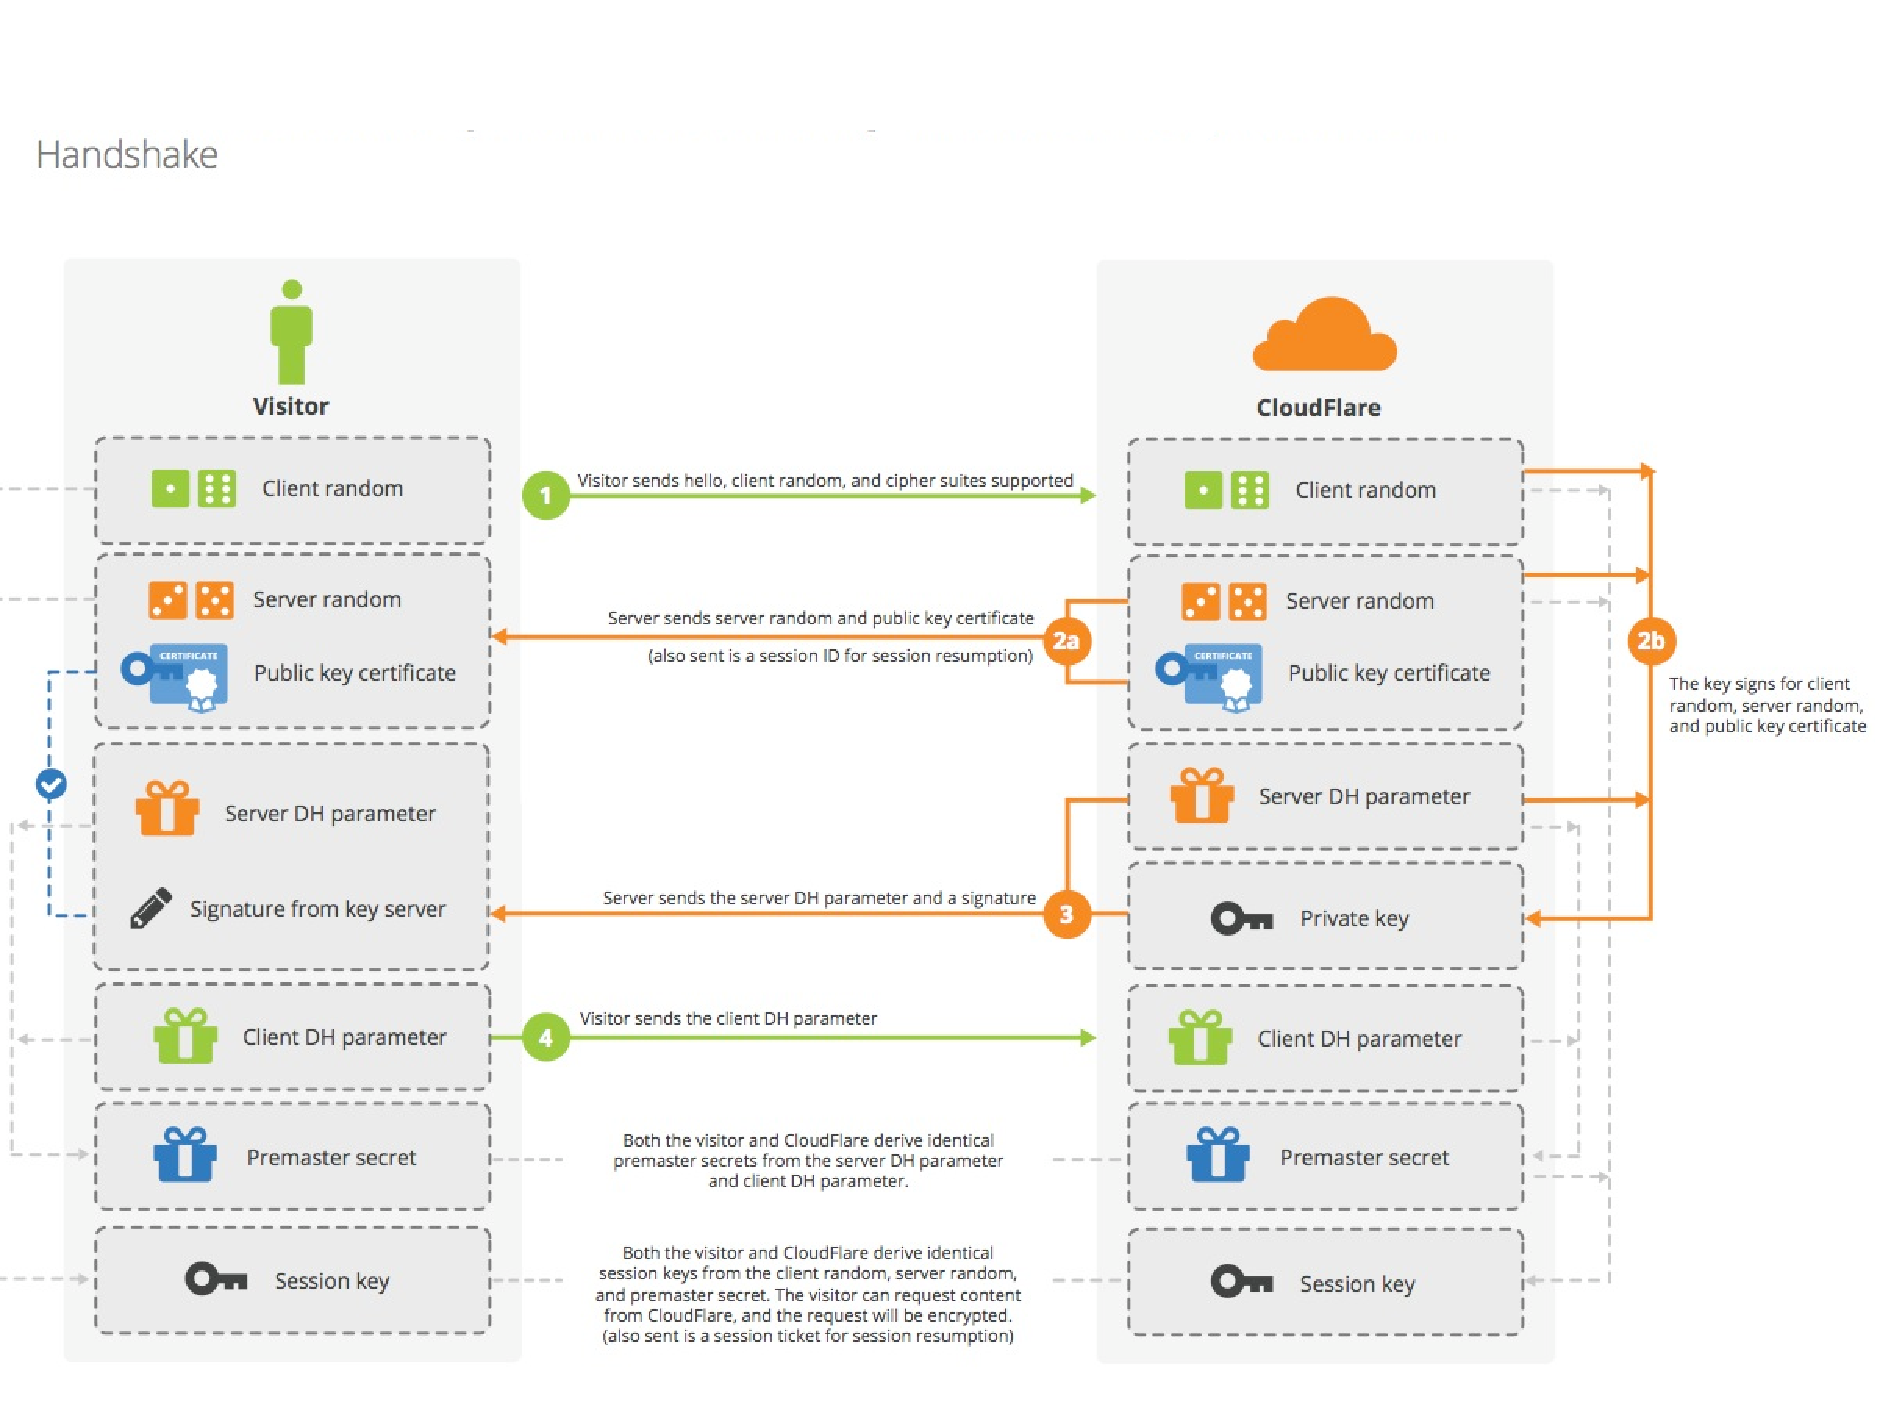
\includegraphics[width=\linewidth]{images/ECDHEhandshake}
\caption[TLS handshake with ECDHE]{TLS handshake with ECDHE for key exchange (image from \cite{tlsdhhandshake})}
\label{fig:tls_handshake}
\end{figure}

In the first phase, the client gives its version together with a list of algorithms for encryption and authentication called cipher suites. The client also gives to the server a random token to be used later. The server will then choose among the ones proposed: the version and the cipher suite to be used for the rest of the communication. A random server token is also included in the reply. In addition, the server may provide a session ID which can be used later for session resumption.

In a separated message, the server also provides its certificate to the client. It contains enough information for the latter to be able to verify server's identity. The certificate is generally emitted by a certification authority which is known by the client.

The next step comes with the server providing its DH parameters. In the case of ephemeral keys, the DH parameters must be different for every session. A digital signature using RSA with the server's private key is also included. The signature is computed not only on the information carried in this packet but also on all the previous exchanged messages. This is needed to prevent a man-in-the-middle attack. The genuine server is supposed to be the only one to hold the private key.

Then, the client provides its own DH parameters. Note that no signature is provided in this case as it is only optional to authenticate the client. Indeed, in some applications such as websites, this is not a requirement. After this step, both client and server can deduce the \textit{PreMasterSecret} and thus the master key with the random tokens exchanged before.

All messages following the handshake (containing application data) will be encrypted with symmetric cryptography using the keys deduced from the master key for this particular session. This will ensure the confidentiality. The two other objectives, authenticity and integrity of the messages, are ensured by a keyed-hash message authentication code (HMAC). It is generated as a hash on the content of the packet but the hash algorithm also integrates the secret key. Any cryptographic hash function can be used for this purpose but it is recommended to use at least \texttt{SHA256}. The choice of this function is also negotiated during the client hello, server hello phase. Even if it is better to first encrypt and then MAC the output as stated in \cite{bellare2000authenticated}, TLS works in reverse order for historical reasons. Currently people think it was a very bad idea from a security point of view and a RFC \cite{rfc7366} was published last year to push for the adoption of the encrypt-then-MAC technique on existing systems. It will probably be part of the TLS 1.3 RFC \cite{draft-tls13} to switch definitely to this better practice.

To prevent malicious replays disturbing the normal communication, TLS authenticates each packet with the associated sequence number. The sequence number is incremented for every packet sent but separately for each direction. Therefore each host has two counters: one for the packets sent and a second one for the packets received.

Thanks to a reliable transport protocol, these counters must never be transmitted explicitly because each host can compute them. As a consequence, if an attacker tries to replay packets, they will simply be rejected because the HMAC will not match with the most recent sequence number.

\subsection{Differences between TLS and DTLS}

\subsubsection{Unreliability}

The unreliability brought by UDP causes problems if we apply TLS over datagrams without any modification.

As we explain in the previous section, TLS uses implicit sequence numbers to authenticate packets. If a loss or a reordering occurs, then the sequence number considered by the receiving host will be wrong and the integrity check will fail. To solve this problem, DTLS modifies the record layer and adds a new field to carry the sequence number in every packet. The DTLS 1.2 record layer is presented on Listing \ref{lst:dtls-record}.

\addtypes{ContentType, ProtocolVersion, uint16, uint48, opaque}
\begin{lstlisting}[caption=DTLS record layer, label=lst:dtls-record]
struct {
   ContentType type;
   ProtocolVersion version;
   uint16 epoch;                                    // New field
   uint48 sequence_number;                          // New field
   uint16 length;
   opaque fragment[DTLSPlaintext.length];
 } DTLSPlaintext;
\end{lstlisting}


Epoch is used by endpoints to identify the keys used to protect the payload. The epoch is incremented by one once a \texttt{changeCipherSpec} is sent. Initially, the epoch is set to 0 for the handshake and the following \texttt{changeCipherSpec} will be the first message being part of the next epoch. The sequence number is set back to 0 once a new epoch has started. Due to the risks of retransmission or reordering, the endpoint need a way to know which set of keys were used to crypt the payload, because it cannot simply assume it is the latest negotiated keys. This need is fulfilled thanks to the epoch field.

Another problem raised by unreliability is the fact that in TLS the handshake has to follow a particular order and if not the connection is simply aborted. This is clearly incompatible with losses and retransmissions. To handle potential losses in the handshake phase, implementation must retransmit the last packet after a given time if no answer has been received from the other host (see \cite{rfc6347} Section 4.2.4).

To deal with possible reordering, all handshake messages have a given sequence number. So if a message is received before another one, the first message must be queued for further processing.

\subsubsection{Messages size}

The message size is a potential issue because TLS (and thus DTLS) messages can be as large as $2^{24}-1$ bytes while UDP datagrams are often limited to $1500$ bytes. Therefore, each DTLS handshake message may be fragmented over several DTLS records and then rebuilt. One fragment must fit in a single IP datagram to avoid IP fragmentation.

The benefits to this requirement are stated in the original DTLS paper \cite{modadugu2004design} :
\begin{itemize}
\item The DTLS layer does not need to buffer partial records, host memory can be used more efficiently.
\item It is quite possible that datagrams carrying the remaining record fragments are lost, in which case the received fragments are useless and cannot be processed.
\item Buffering record fragments would unnecessarily complicate a DTLS implementation without providing any obvious benefit.
\end{itemize}

Note that even if IP fragmentation occurs, DTLS will still operate correctly on top of re-assembly since it is transparently handled by the kernel.

The TLS handshake message is modified as shown on Listing \ref{lst:dtls-handshake}. The handshake message following this structure is also encapsulated into the record layer presented on Listing \ref{lst:dtls-record}.

\addtypes{HandshakeType, uint16, uint24, case, select}
\begin{lstlisting}[caption=DTLS handshake message, label=lst:dtls-handshake]
   struct {
     HandshakeType msg_type;
     uint24 length;
     uint16 message_seq;                               // New field
     uint24 fragment_offset;                           // New field
     uint24 fragment_length;                           // New field
     select (HandshakeType) {
       case hello_request: HelloRequest;
       case client_hello:  ClientHello;
       case hello_verify_request: HelloVerifyRequest;  // New type
       case server_hello:  ServerHello;
       case certificate:Certificate;
       case server_key_exchange: ServerKeyExchange;
       case certificate_request: CertificateRequest;
       case server_hello_done:ServerHelloDone;
       case certificate_verify:  CertificateVerify;
       case client_key_exchange: ClientKeyExchange;
       case finished: Finished;
     } body;
   } Handshake;
\end{lstlisting}

\subsubsection{Anti-Replay strategy}

In TLS, sequence numbers follow sequentially and a packet cannot be replayed because the HMAC verification will fail immediately. Such a drastic solution cannot be applied in DTLS because reordering or losses may occur. The DTLS 1.2 RFC \cite{rfc6347} sec. 4.1.2.6 describes the procedure to avoid replay using a sliding window. This strategy considers packets as valid even if they have been delayed or reordered while they are relatively close from the latest packets received. At the same time, the implementation must remember the packets received inside the sliding window and silently discard the replayed packets. Therefore, the MAC verification will only be done if the packets have not been received before, otherwise an undesirable packet is discarded at the record layer stage.

\subsubsection{Anti-DoS for the handshake}

In order to prevent DoS (Denial of Service) attacks, DTLS adds an additional step in comparison with the TLS handshake. Indeed, an attacker could send a lot of \texttt{ClientHello} messages and the server will have to keep a state for each of them, rapidly increasing the memory needed. Instead, the first \texttt{ClientHello} will not directly trigger a \texttt{ServerHello} but a \texttt{HelloVerifyRequest}. This message only carries the protocol version and a cookie as presented in Listing \ref{lst:dtls-helloverify}. This cookie must be retransmitted in the next Client Hello message. As we can seen on Listing \ref{lst:dtls-clienthello}, a new field has effectively been added to the \texttt{ClientHello} message.

\addtypes{ProtocolVersion, opaque}
\begin{lstlisting}[caption=DTLS HelloVerifyRequest message, label=lst:dtls-helloverify]
struct {
 ProtocolVersion server_version;
 opaque cookie<0..2^8-1>;
} HelloVerifyRequest;
\end{lstlisting}


\addtypes{ProtocolVersion, opaque, Random, SessionID, CipherSuite, CompressionMethod}
\begin{lstlisting}[caption=DTLS ClientHello adapted message, label=lst:dtls-clienthello]
struct {
 ProtocolVersion client_version;
 Random random;
 SessionID session_id;
 opaque cookie<0..2^8-1>;                             // New field
 CipherSuite cipher_suites<2..2^16-1>;
 CompressionMethod compression_methods<1..2^8-1>;
} ClientHello;
\end{lstlisting}

The additional \texttt{HelloVerifyRequest} message is also a counter measure against amplification attacks. Such attacks are trying to redirect traffic to overload a particular target by using an other server to generate bigger messages. These attacks are possible if the generated message is larger than the one triggering it. It is the case with DNS since the reply is larger than the request if a particular domain has multiple DNS records. It becomes then a vector for DoS attacks (see Figure \ref{fig:amp_attack} taken from \cite{dns-amp}).


\begin{figure}[!ht]
\centering
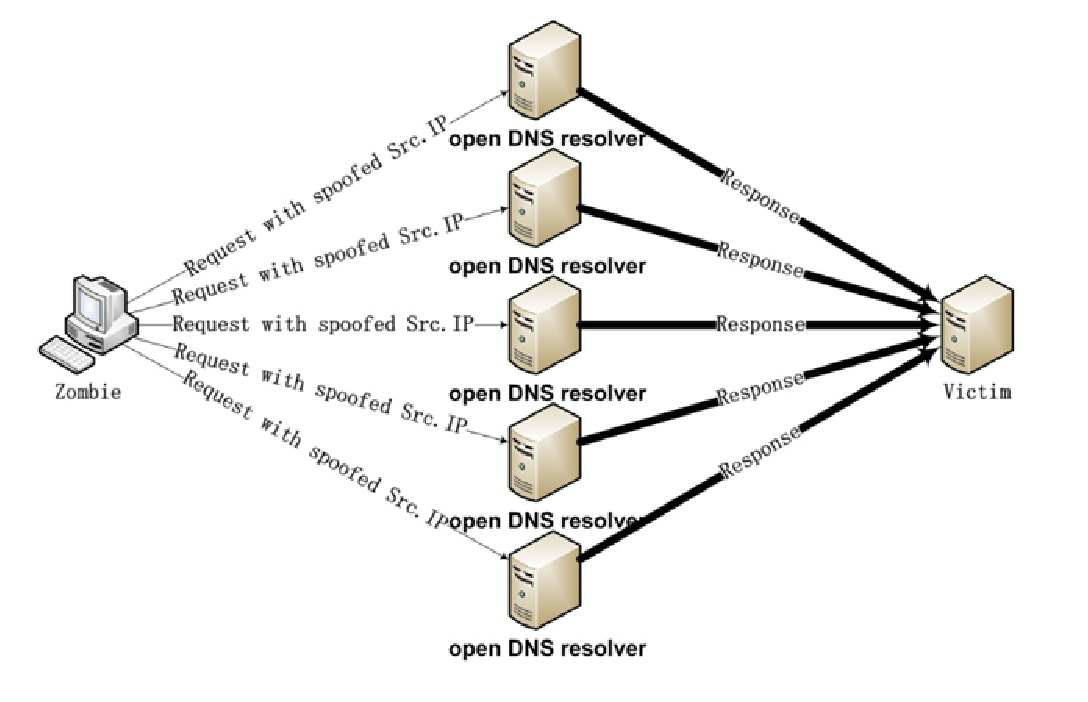
\includegraphics[width=\textwidth]{images/amplificationattacks}
\caption{Example of amplification attack with DNS}
\label{fig:amp_attack}
\end{figure}

For DTLS, the \texttt{ServerHello} is not larger than the \texttt{ClientHello} but amplification attack could still be possible (without the \texttt{HelloVerifyRequest}). Indeed, other messages are sent together with the \texttt{ServerHello}, including the one carrying the certificate (that could be quite large). Therefore, the additional step introduced with the \texttt{HelloVerifyRequest} (which is relatively small) prevents this kind of attack because the client has to prove it can answer at this address.

When the client sends its first \texttt{ClientHello}, the cookie field is initially empty. The server will then generate a new cookie which allows for a stateless exchange. It sends the \texttt{HelloVerifyRequest} with the cookie and doesn't remember anything about the client\footnote{This is indeed an exception to the retransmission measures. A \texttt{HelloVerifyRequest} will never be retransmitted, the client must first send another \texttt{ClientHello}.}. The DTLS server must generate cookies in such a way that they can be verified without retaining any per-client state on the server. A way to compute it is given in the RFC6347 section 4.2 \cite{rfc6347}:

\begin{lstlisting}
Cookie = HMAC(Secret, Client-IP, Client-Parameters)
\end{lstlisting}

The \texttt{Secret} is random and generated by the server. It could be periodically refreshed to invalidate previous cookies. Once a \texttt{ClientHello} has been received with a cookie, the server recomputes it and if both match, the connection can continue as in TLS with a \texttt{ServerHello} message.

\section{Typical DTLS communication}

\subsection{Handshake}

\begin{figure}[!h]
\centering
\begin{msc}[r]{DTLS Handshake}

\setlength{\instfootheight}{0em}
\setlength{\instheadheight}{0em}
\setlength{\instdist}{0.7\linewidth}
\setlength{\levelheight}{3em}

\declinst{client}{Client}{}
\declinst{server}{Server}{}

\mess{Client Hello}[t]{client}[0.3]{server}[1]
\nextlevel
\mess{Hello Verify Request}[t]{server}[0.3]{client}[1]
\nextlevel
\mess{Client Hello (w/ cookie)}[t]{client}[0.3]{server}[1]
\nextlevel
\mess{Server Hello}[t]{server}[0.5]{client}[1]
\nextlevel
\mess{Certificate}[t]{server}[0.5]{client}[1]
\nextlevel
\mess{Server Key Exchange}[t]{server}[0.5]{client}[1]
\nextlevel
\mess{Server Hello Done}[t]{server}[0.3]{client}[1]
\nextlevel
\mess{Client Key Exchange}[t]{client}[0.3]{server}[1]
\nextlevel
\mess{Change Cipher Spec}[t]{client}[0.3]{server}[1]
\nextlevel
\mess{Change Cipher Spec}[t]{server}[0.3]{client}[1]
\nextlevel
\nextlevel
\end{msc}
\caption{DTLS handshake with ECDHE-RSA cipher suite}
\label{fig:dtls-handshake}
\end{figure}


Figure \ref{fig:dtls-handshake} depicts a typical handshake with authentication of the server only and the ECDHE-RSA cipher suite\footnote{It means that Elliptic Curve Diffie-Hellman ephemeral is used for the key exchange and RSA for the signature.}. All messages before the \texttt{ChangeCipherSpec} are part of epoch 0. Their role is to negotiate the algorithms that will be used to compute the master key. The \texttt{Client Hello} has also the role to carry potential extensions supported by the client. If the server supports them as well, it will include them in the following \texttt{Server Hello} message. This is also where we chose to advertise our MPDTLS extension as explained in Chapter \ref{chap:design}.

The only difference with TLS (Section \ref{sec:tls}) is the presence of a second \texttt{ClientHello}. The first one is sent with no cookie and the second one must repeat the cookie received with the \texttt{HelloVerifyRequest}. Then the server confirms the cipher suite to be used through the \texttt{ServerHello} and directly sends its certificate and its ephemeral public key\footnote{In the case of ECDHE, it consists of the public DH parameters. Namely the domain parameters to define a particular curve.} including a signature of all previous exchanged messages. Finally the server sends the \texttt{ServerHelloDone} to explicitly say that the handshake is finished on its side.

Thereafter the client must also send its DH ephemeral public key. At this point, both parties have all the elements in their hands to compute the premaster secret. Note that unlike RSA, the secret is never communicated through the channel. With the random information exchanged through the \texttt{ClientHello} and \texttt{ServerHello}, each host can also compute the master key on its side. Consequently each peer will use this key to derive the set of keys used to communicate in the next epoch. The first messages of epoch 1 are the \texttt{ChangeCipherSpec} messages. They explicitly mark the separation between the handshake and the rest of the communication. Even if they are technically separated from the handshake, they are still considered as being part of it from a conceptual point of view.


\subsection{Application data}

Once the handshake has been completed, the peers can exchange Application Data packets. They are first encrypted and authenticated using the parameters negotiated earlier, then encapsulated into a Record Layer (Listing \ref{lst:dtls-record}).

DTLS doesn't bring any additional guarantee concerning the reliability of the link. As shown in Figure \ref{fig:dtls-data}, packets may be lost on the way and the application must deal with it. The sequence number for each message is indicated between chevrons. Sequence numbers are carried in clear inside the record layer, so each host knows how to verify the MAC and authenticate the packet.

\begin{figure}[!h]
\centering
\begin{msc}[r]{DTLS communication}

\setlength{\instfootheight}{0em}
\setlength{\instheadheight}{0em}
\setlength{\instdist}{0.7\linewidth}
\setlength{\levelheight}{3em}

\declinst{client}{Client}{}
\declinst{server}{Server}{}

\mess{Application Data <1>}[t]{client}[0.3]{server}[1]
\nextlevel
\mess{Application Data <1>}[t]{server}[0.3]{client}[1]
\nextlevel
\nextlevel
\lost[r]{Application Data<2>}[t]{}{client}[3]
\nextlevel
\mess{Application Data<3>}[t]{client}[0.3]{server}[1]
\nextlevel
\mess{Application Data<2>}[t]{server}[0.5]{client}[1]
\nextlevel
\nextlevel
\end{msc}
\caption{DTLS application data exchange}
\label{fig:dtls-data}
\end{figure}

\section{Use cases}

\label{sec:dtls-usage}

DTLS can be used almost everywhere UDP is used. We can think about applications such as VoIP (Voice over IP), multimedia, online gaming. Every application that wants to secure its communication but still benefit from faster transmission time of UDP may take advantage of using DTLS.

Of course the application has to cope with losses or reordering, but this is already the case for real time communication. As regards telephony, blank sounds replace the missing packets. For online gaming, high speed communication between the server and the client is needed to determine the character's position for instance. But if one packet is lost, the position can be determined by the next packet and the application will not be disturbed.

For video streaming applications, techniques are used to introduce a slight redundancy at the codec level in such a way that if some packets are lost, one frame may be missing but at least the video is still watchable\footnote{Of course, the application must a use a proper codec and compression method.}. It is also possible to introduce a small buffer to handle reordering.

In a recent Internet draft \cite{dtls-as-subtransport}, companies are trying to make DTLS the default sub-transport protocol for all application-level protocols when security is needed. This will raise DTLS to the rank of "good practice" for secured communications.

Another important use case for DTLS comes with its integration in WebRTC\footnote{\url{http://www.webrtc.org/}}. This is an open project which has an objective to bring real time communications to browsers and mobile applications via simple APIs. In this context, DTLS has been chosen to ensure the communication between two peers (i.e. browsers or mobile apps). The internet draft describing the security architecture of WebRTC \cite{ietf-rtcweb-security-arch} proposes to use SRTP over DTLS for multimedia communications and DTLS alone for any other kind of data. Figure \ref{fig:webrtc} is taken from a presentation \cite{rescorla2011proposed} made by E.Rescorla and shows how the connection is set up in this proposed design.  

\begin{figure}[!ht]
\centering
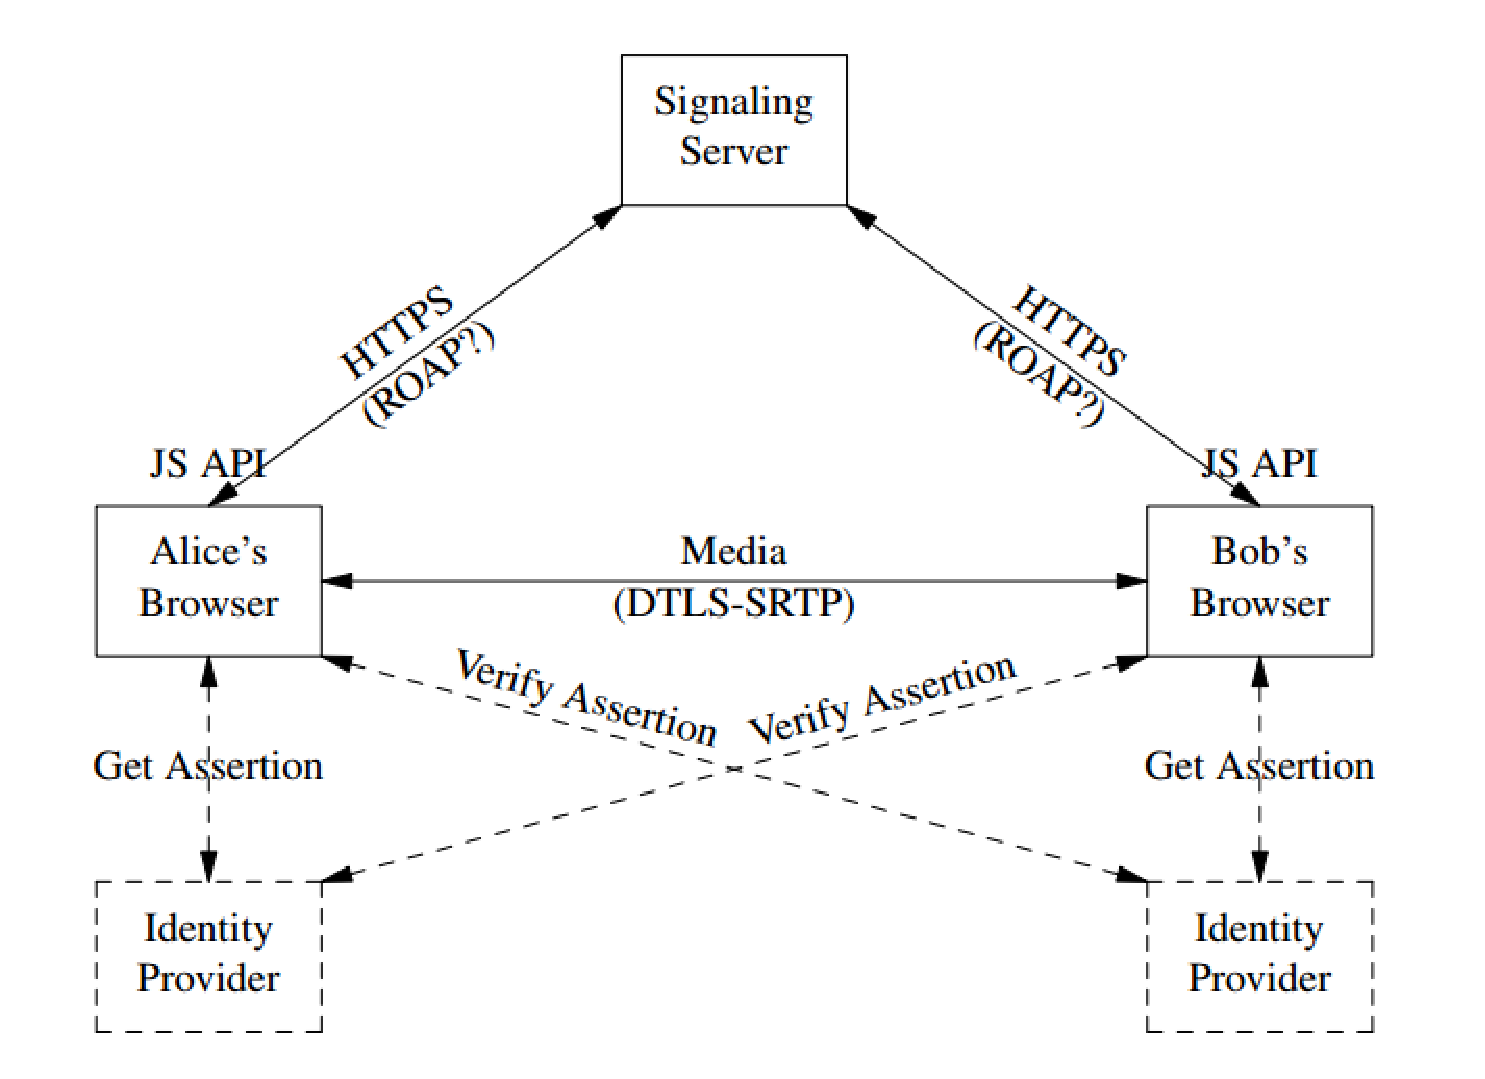
\includegraphics[width=0.9\textwidth]{images/webrtc.eps}
\caption{Proposed design for WebRTC security architecture}
\label{fig:webrtc}
\end{figure}

By the peer to peer nature of this application, a signalling server is needed to act as a "rendez-vous" point and to perform NAT traversal. Then the handshake can take place and identity providers issue and verify certificates. Finally all data are transmitted through the DTLS transmission and multiple SRTP sessions can use the same DTLS session. 

To sum up, all these applications may benefit from using DTLS but also MPDTLS as it will allow more resilience and better performances. We will demonstrate this point in the following chapters.

\section{Security considerations}
\label{sec:tls-sec}

Most of the security considerations are the same as those of TLS 1.2 \cite{RFC5246} since DTLS is only an adaptation of TLS for unreliable transport protocols.

The attacks known for TLS could theoretically be used for DTLS as well. This is the case for the "secure renegotiation". As a reminder, this vulnerability allows an attacker who can hijack a HTTPS connection to add custom request to a communication between the client and the web server. Even if the attacker cannot retrieve the content of the communication, it can still have dramatic consequences. As depicted on Figure \ref{fig:tls-reneg} taken from \cite{tls-reneg}, an attacker can inject bank orders and then trigger the renegotiation with a real client. The bank order is only delayed and when the renegotiation is completed, it is executed before anything else. The best solution up to know is to disable by default this feature or to implement the extension described in \cite{rfc5746}.

\begin{figure}[!ht]
\centering
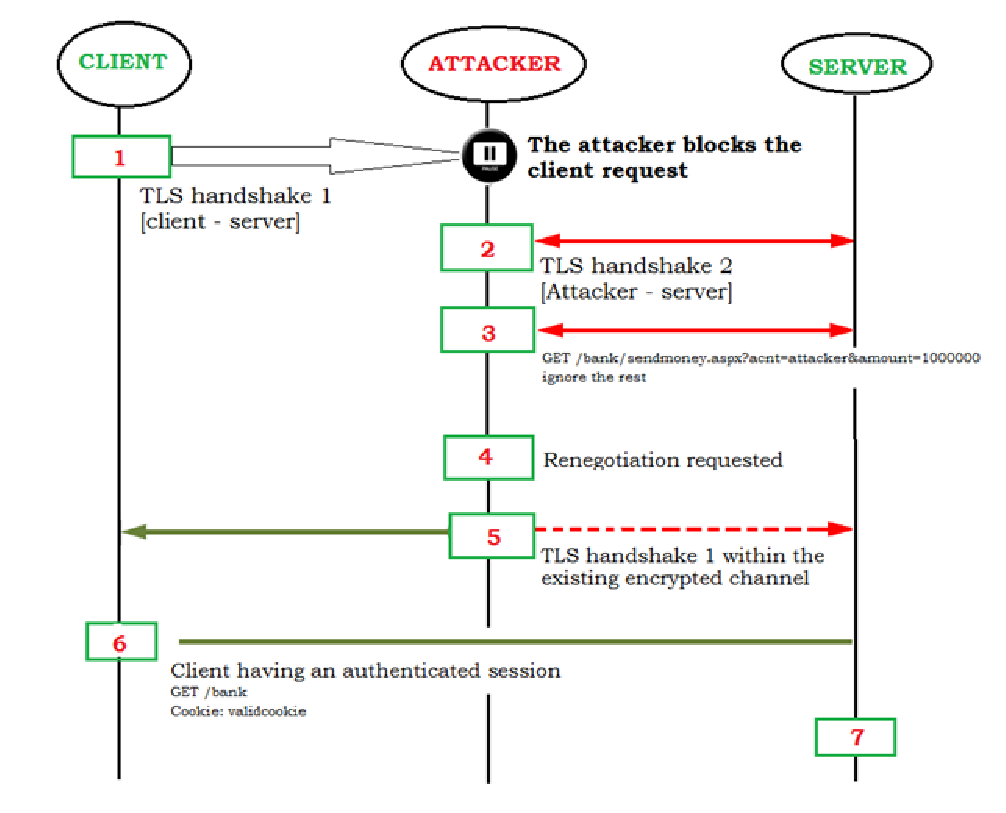
\includegraphics[width=0.8\textwidth]{images/TLSrenegotiation}
\caption{TLS renegotiation vulnerability}
\label{fig:tls-reneg}
\end{figure}

Other attacks could also be applied to DTLS and be more efficient on DTLS than on TLS, namely the DoS attacks. Two main categories can be identified :

\begin{itemize}
\item The blind DoS : packets are being transmitted with a spoofed IP address to redirect the traffic to another target (amplification attack) or to simply not diclose the IP address of the attacker. They are called blind because the attacker will never receive any answer from the server. They are made easier with UDP because no handshake is needed with the server.
\item Computational DoS : the attacker can reply to certain messages but will try to optimize the ratio between the work he has to do and the work he is asking to the server.
\end{itemize}

Blind DoS are made impossible in TLS because the attacker must first complete the TCP handshake and thus prove he can answer at this address. As presented earlier, the introduction of the \texttt{Hello Verify Request} will prevent this kind of attack for DTLS too.  Although it is not a strict requirement to implement this feature in DTLS (\cite{rfc6347} Section 5), it is strongly recommended for DTLS servers  unless there is a good reason to think that no amplification is possible in their environment.

Nevertheless the second type can still be used to disturb a server running DTLS or even TLS. As explained by E. Rescorla in \cite{tls-dos}, nothing is done at the design level to prevent these kind of attacks because it would imply putting a lot of work on the client side. It is generally a bad idea for performances. Moreover, the attackers are often using infected computers of casual people to launch DoS attacks. Therefore they have a lot of CPU power available anyway.

\section{Heartbeat extension}

The heartbeat extension is unfortunately known for the famous heartbleed bug\footnote{\url{http://heartbleed.com/}} detected in April 2014. Every server using OpenSSL at this time was vulnerable and part of the memory could be retrieved (including private keys, passwords\dots). It is important to note that the error came from the implementation of the extension inside OpenSSL and not from the standard itself.

Anyway, this extension can be really useful to assess the availability of a link and also provides a keep-alive feature. It is quite simple but it also allows for extensibility and new messages as stated in RFC6520 \cite{rfc6520}. The structure of a heartbeat message is presented on Listing \ref{lst:hb-msg}. This will take place on top of the Record Layer (Listing \ref{lst:dtls-record}). The advertisement of this extension is made through a Hello extension. It also defines the behavior of the hosts upon the reception of Heartbeat messages.

\addtypes{HeartbeatMessageType}
\begin{lstlisting}[caption=Heartbeat message, label=lst:hb-msg]
struct {
  HeartbeatMessageType type;
  uint16 payload_length;
  opaque payload[HeartbeatMessage.payload_length];
  opaque padding[padding_length];
} HeartbeatMessage;
\end{lstlisting}

For now, only two types of Heartbeat messages are in use : \texttt{Heartbeat Request} and \texttt{Heartbeat Response}. The response must contain the same payload as the one in the request triggering it. A simple exchange is presented on Figure \ref{fig:heartbeat}.

\begin{figure}[!h]
\centering
\begin{msc}[r]{Heartbeat request/response}

\setlength{\instfootheight}{0em}
\setlength{\instheadheight}{0em}
\setlength{\instdist}{0.7\linewidth}
\setlength{\levelheight}{3em}

\declinst{host1}{Host 1}{}
\declinst{host2}{Host 2}{}

\lost[r]{Heartbeat Request}[t]{}{host1}[3]
\nextlevel
\mess{Heartbeat Request}[t]{host1}[0.3]{host2}[1]
\nextlevel
\mess{Heartbeat Response}[t]{host2}[0.5]{host1}[1]
\nextlevel
\nextlevel
\end{msc}
\caption{Heartbeat requests and responses}
\label{fig:heartbeat}
\end{figure}

Other messages may be implemented since a new IANA section has been opened to register the different \texttt{HeartbeatMessageType}. Indeed, as you will see in the Chapter \ref{chap:implementation}, we have designed a new type of message used to transmit a timestamp.

\appendix


\bibliographystyle{unsrt}
\bibliography{articles,rfcs}

\end{document}

